% A basic LaTeX document for an assignment

% If you want the title to appear on a separate
% page, change notitlepage to titlepage
\documentclass[11pt,a4paper,titlepage]{article}
\usepackage[utf8]{inputenc}
\usepackage[T1]{fontenc}
% If your hand-in is in icelandic change english to icelandic
% Note: This has nothing to do with Icelandic characters, they
% can always be used. This just tells other packages what 
% language you are using and changes the hyphenation used by LaTeX
% If icelandic is selected, a shorthand, "` and "', is also included
% for Icelandic quotation marks. They can also obtained by using 
% ,, and ``
\usepackage[icelandic]{babel}
\usepackage{amsmath, amsthm, amssymb, amsfonts}
\usepackage{graphicx}
\usepackage{enumerate}
% To use the whole A4-page
% See: ftp://ftp.tex.ac.uk/tex-archive/macros/latex/contrib/geometry/geometry.pdf
% and http://en.wikibooks.org/wiki/LaTeX/Document_Structure
\usepackage{geometry}
% For header and footer
% See: ftp://ctan.tug.org/tex-archive/macros/latex/contrib/fancyhdr/fancyhdr.pdf
% and http://en.wikibooks.org/wiki/LaTeX/Document_Structure
\usepackage{fancyhdr}
% For prettier tables
% See: http://ctan.mackichan.com/macros/latex/contrib/booktabs/booktabs.pdf
% and  http://en.wikibooks.org/wiki/LaTeX/Tables
\usepackage{booktabs}
\usepackage[framed,numbered,autolinebreaks,useliterate]{mcode}
\usepackage{wrapfig}
\usepackage{float}

%%%%%%%%%%%%%%%%%%%%%%%%%%% SETUP %%%%%%%%%%%%%%%%%%%%%%%%%%%

% Set the margins of the paper. By default LaTeX uses huge margins
\geometry{includeheadfoot, margin=2.5cm}
% you can also use
% \geometry{a4paper}
% End of margins setup

% Setup header and footer
% Headers

%\pagestyle{fancy} % To get the header and footer
%\chead{\small \textsc{Heimadæmi 7}}
%\rhead{\small \textsc{Guðrún Kristín Einarsdóttir}}
%\lhead{\small \textsc{Ólínuleg bestun}}
% Footers
%\lfoot{Left footer text}
%\cfoot{\thepage} % This is the default behaviour
%\rfoot{Right footer text}

% If you don't want a line below the header or above the footer, 
% change the appropriate header/footerrulewidth to 0pt
\setlength{\headheight}{15.2pt} % This is set to avoid a warning
\renewcommand{\headrulewidth}{0.4pt}
\renewcommand{\footrulewidth}{0.4pt}
% End of header and footer setup


% Setup Problem/Solution environments
\theoremstyle{plain}
\newtheorem{verkefni}{Verkefni}

\theoremstyle{remark}
\newtheorem*{lausn}{Lausn}
% End of Problem/Solution environments setup

%%%%%%%%%%%%%%%%%%%%%%%% END OF SETUP %%%%%%%%%%%%%%%%%%%%%%%%

\titlepage

\begin{document}
\begin{center}


\textsc{Háskóli Íslands}
\end{center}
\vspace*{5cm}



\large {\bf
\begin{center}
\noindent\rule{15cm}{0.4pt}
\textsc{Þróun Hugbúnaðar}\\ \textsc{Hópverkefni 2d}\\ Tri Peaks \\
\noindent\rule{13cm}{0.4pt} \end{center}}
\small
\vspace{5cm}
\begin{center}
Ágúst Ingi Skarphéðinsson\\Guðrún Kristín Einarsdóttir\\Kári Ragnarsson\\Priyaphon Kaengjaroenkasikorn\\ Valur 
Sigurbjörn Pálmarsson
\end{center}
\vspace{5cm}
\begin{center}
\today
\end{center} 

\newpage \normalsize 
\newpage

\section{Virkni kapalsins}

Kapallinn kallast Tri-Peaks og er spilaður með einum spilastokki með 52 spilum. 18 spilum er raðað í borðið þannig að þau myndi þrjá píramída sem skarast (sjá mynd). Afgangurinn af spilunum er svo hafður í stokk á borðinu og efsta spilið lagt út við hliðina á stokknum og myndar það hrúguna sem spilin munu verða lögð ofan á.

\begin{figure}[H]
\centering
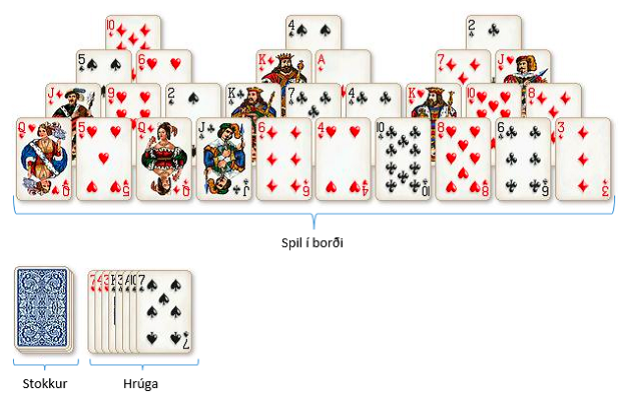
\includegraphics[scale=0.8]{uppstillingTriPeaks.png}
\caption{Uppsetning kapalsins}
\end{figure}

Markmið kapalsins er að flytja öll spilin í borðinu yfir í hrúguna og opna þannig fyrir spilin sem eru ofar í borðinu svo hægt sé að nota þau. Kapallinn er unnin þegar öll spil í borðinu hafa verið færð úr borðinu yfir í hrúguna.

\subsection*{Reglur}

Einungis má hreyfa spil í borðinu sem ekki eru undir öðru spili. Færa má spil yfir á hrúguna ef það hefur einum lægra eða hærra gildi en spilið sem er efst í hrúgunni. Á myndinni fyrir ofan mætti t.d. færa \emph{ATH SETJA INN TAKN} eða \emph{ATH SETJA INN TAKN}  ofaná \emph{ATH SETJA INN TAKN}  í hrúgunni. Auk þess má setjá kóng ofan á ás og ás ofan á kóng. Þegar ekki er hægt að færa fleiri spil úr borðinu á hrúguna er spil dregið úr stokknum og sett efst á hrúguna og þá má færa spil úr borðinu á hrúguna líkt og áður. Þegar stokkurinn hefur klárast og ekki er hægt að færa fleiri spil úr borðinu á hrúguna þá hefur leikurinn tapast. Bónusstig fást þegar öll spilin úr einum píramída hafa verið fjarlægð. Auk þess fást bónusstig fyrir hvert spil sem eftir er í stokknum þegar kapallinn er unninn ásamt því að lokastigin eru háð því hversu hratt kapallinn er kláraður.


\section{Bónusvirkni}

Í þriðju ítruninni var bónusvirkni kapalsins útfærð. Við útfærsluna var miðað við að bæta við virkni sem gerði kapalinn þægilegri og/eða skemmtilegri fyrir notandann. Hér verða taldar upp þær viðbætur sem útfærðar voru.

\begin{itemize}
\item {\bf Hægt að tvísmella á spil í borði} \\
Auk þess sem hægt er að draga spil í borði yfir í hrúguna þá var ákveðið að útfæra virkni þar sem notandi getur tvísmellt á spil í borðinu og þá hreyfist það sjálft yfir í hrúguna. Þetta gerir spilun kapalsins mun þægilegri fyrir notandann þar sem hann þarf ekki sífellt að draga spil yfir borðið. 

\item {\bf Spil hreyfist úr borði í hrúgu með animation} \\ 
Spilið er fært um helming vegalengdarinnar að hrúgunni í hverri lykkju leiksins. Þannig fæst "smooth" færsla á spilinu yfir í hrúguna sem gefur betri upplifun en ef spilið mydni birtast samstundis í hrúgunni. 

\item {\bf Hljóð} \\
Til þess að gera kapalinn skemmtilegri í spilun var bætt við hljóðum. Spilahljóð heyrist þegar spil er fært úr borði í hrúgu eða úr stokk í hrúgu. Þegar notandi tapar kaplinum er spilað sorglegt lag en þegar notandi vinnur er glaðlegt lag spilað. 

\item {\bf Gefa vísbendingar um mögulegar færslur} \\
Bætt var við virkni sem gerir notanda kleift að fá vísbendingar um hvaða spil í borði má færa á hrúguna. Til þess að sjá hvaða spil má hreyfa smellir notandi á H á lyklaborði og þá verða öll ólögleg spil í borðinu gegnsæ en þau sem eru lögleg haldast óbreytt. Þannig má sjá fljótt og greinilega hvaða spil er hægt að færa. 

\item {\bf Bakgrunnsmynd} \\
Til þess að gera leikinn meira aðlaðandi og skemmtilegri í spilun var sett mynd í bakgrunninn. Passað var að velja ekki mynd sem tæki athygli notanda frá kaplinum heldur að hún myndi aðeins styðja við grafík kapalsins. 

\item {\bf Animation þegar spil er dregið} \\
Spilið er fært um helming vegalengdarinnar að hrúgunni í hverri lykkju leiksins. Þannig fæst "smooth" færsla á spilinu yfir í hrúguna sem gefur betri upplifun en ef spilið myndi birtast samstundis í hrúgunni. 

\item {\bf Spil verða óvirk þegar leikur er búinn} \\
Þegar notandi hefur tapað kaplinum þá verða öll spil sem eftir eru í borðinu gegnsæ svo augljóst er að ekki er hægt að hreyfa þau. Þetta er gert til þess að hafa skýr skil á milli þess þegar kapallinn er í spilun og þegar hann er búinn.

\item {\bf Animation þegar spil eru gefin í borð} \\
Til þess að hressa upp á kapalinn þegar leikur hefst var útært animation fyrir það þegar spilin eru gefin í borð. Þá er byrjað á að gefa efsta spilið til vinstri og þaðan farið til hægri og niður þar til öll spilin eru komin í borð. Hvert spil hreyfist hálfa vegalengd frá stokknum að sínum stað í hverri lykkju leikjarins og fæst þannig "smooth" færsla á hverju spili.

\end{itemize}


\section{Framvinda verkefnis}

Við upphaf verkefnisins höfðum við lært töluvert af fyrra verkefninu, t.d. varðandi tímaáætlun þar sem við áttum það til að vanáætla tíma á verkþætti. Þá gleymdist oft að taka til greina tíma sem getur farið í að finna villur í kóða og ná í nauðsynlega pakka fyrir Python sem getur verið tímafrekt. Í byrjun þessa verkefnis reyndum við því að passa okkur á því að vanáætla ekki tíma fyrir verkþætti ásamt því að byrja strax á að skipuleggja verkþættina betur. Þetta skilaði sér svo í því að við lentum ekki í eins mikilli tímaþröng í þessu verkefni.

\subsection*{Ítrun 1}
Í fyrstu ítrun verkefnisins var lögð áhersla á að ná allri virkni kapalsins í lag. Notendasögur fyrstu ítrunar fólu því í sér næstum alla virkni kapalsins en gerðu ekki ráð fyrir neinni grafík. Það náðist að klára allar þær notendasögur í ítruninni og í fyrstu útgáfu af kaplinum var hann spilaður í skel þar sem notandi þurfti að slá inn skipanir til að færa spil. Ekkert var byrjað að skoða grafíska notendaviðmótið í þessari ítrun. Einingapróf voru útfærð hér sem dekkuðu sem mest af virkni kapalsins og stóðust þau flest.

\subsection*{Ítrun 2}

Í annarri ítrun var byrjað að skoða grafíska viðmótið og gekk það betur en við bjuggumst við fyrirfram. Hópurinn lenti þó í ýmsum vandræðum með að ná í pygame pakkann í Python sem þurfti til að gera viðmótið. Það hófst þó allt á endanum og forritun grafíska viðmótsins gekk áfallalaust.

\subsection*{Ítrun 3}

Þriðja ítrunin fór aðallega í áframhaldandi þróun á grafíska viðmótinu og útfærslu á bónusvirkni kapalsins. Einnig fór tími í þriðju ítrun í prófanir á kaplinum, bæði kerfisprófanir og útfærslu einingaprófana.

\bigskip

Við upphaf verkefnisins var lagt upp með eftirfarandi notendasögur:

\begin{itemize}
\item Notandi vill geta hafið nýjan leik
\item Notandi vill geta hætt í leiknum hvenær sem er
\item Notandi vill geta séð reglur leiksins
\item Notandi vill geta dregið spil úr stokki
\item Notandi vill geta dregið spil úr borði yfir í hrúgu
\item Notandi vill geta byrjað upp á nýtt þegar hann vill
\item Notandi vill geta séð þegar hann vinnur eða tapar
\item Notandi vill geta séð stigin sín
\item Notandi vill geta séð leiktíma
\item Notandi vill geta séð highscore töflu
\item Notandi vill geta séð hversu mörg move hann hefur gert
\end{itemize}

Að verkefni loknu hafa allar notendasögurnar verið útfærðar auk þess sem nokkrar notendasögur bættust við sem bónusvirkni.

\section{Vinnuframlag nemenda}

Hér að neðan er stutt lýsing á því hverju nemendur hópsins komu að í framkvæmd þessa verkefnis.

\subsection*{Ágúst Ingi}

\begin{enumerate}
\item
\item
\item
\item
\end{enumerate}

\subsection*{Guðrún Kristín}

\begin{enumerate}
\item Forritun klasa fyrir spil, spilastokk, kapal og viðmót ásamt aðferðum þeirra
\item Forritun falla sem sjá um virkni kapalsins
\item Forritun grafísks notendaviðmóts
\item Forritun bónusvirkni
\end{enumerate}

\subsection*{Kári}

\begin{enumerate}
\item Hluti af grafísku viðmóti
\item Einingapróf
\item Prófanir
\item Leiðréttingar
\end{enumerate}

\subsection*{Priyaphon}

\begin{enumerate}
\item
\item
\item
\item
\end{enumerate}

\subsection*{Valur Sigurbjörn}

\begin{enumerate}
\item
\item
\item
\item
\end{enumerate}

	
\end{document}

